%------------------------------------------------------------------------------
% $Id: easychair.tex,v 1.50 2011/08/07 19:46:18 mokhov Exp $
%

% Select appropriate paper format in your document class as
% instructed by your conference organizers.
%
% The available formats are 'letterpaper' and 'a4paper' with
% the former being the default if omitted as in the example
% below.
%
\documentclass{easychair}
%\documentclass[debug]{easychair}
%\documentclass[debug,verbose]{easychair}
%\documentclass[withtimes,notimes]{easychair}
%\documentclass[notimes]{easychair}
%\documentclass[withtimes]{easychair}
%\documentclass[a4paper]{easychair}
%\documentclass[notimes,custompaper,lmargin=1cm,rmargin=2cm,tmargin=.5cm,bmargin=1.5cm,debug]{easychair}
%\documentclass[notimes,custompaper,lmargin=1cm,rmargin=2cm,tmargin=.5cm,bmargin=1.5cm,debug]{easychair}
%\documentclass[thesis]{easychair}

% This provides the \BibTeX macro
\usepackage{doc}
\usepackage{makeidx}

% In order to save space or manage large tables or figures in a
% landcape-like text, you can use the rotating and pdflscape
% packages. Uncomment the desired from the below.
%
% \usepackage{rotating}
% \usepackage{pdflscape}

% If you plan on including some algorithm specification, we recommend
% the below package. Read more details on the custom options of the
% package documentation.
%
% \usepackage{algorithm2e}


% Some of our commands for this guide.
%
\newcommand{\easychair}{\sf{easychair}}
\newcommand{\miktex}{MiK{\TeX}}
\newcommand{\texniccenter}{{\TeX}nicCenter}
\newcommand{\makefile}{\texttt{Makefile}}
\newcommand{\latexeditor}{LEd}

%%%%%%%%%%%%%%%%%%%%%%%%%%%%%%%%%%%%%%%%%%
%
% Contributors: 
%
% Serguei Mokhov
% Peter Grogono 
% Joey Paquet (1993-2007)
% John Plaice (1993-1999)
%
%
% Cross-reference commands
% Peter Grogono and Serguei Mokhov
%
% Lucid semantics commands
% John Plaice and Joey Paquet
%
%%%%%%%%%%%%%%%%%%%%%%%%%%%%%%%%%%%%%%%%%%

\newcommand{\xp}[1]{page~\pageref{#1}}
\newcommand{\xf}[1]{Figure~\ref{#1}}
\newcommand{\xfp}[1]{Figure~\ref{#1}, \xp{#1}}
\newcommand{\xs}[1]{Section~\ref{#1}}
\newcommand{\xsp}[1]{Section~\ref{#1}, \xp{#1}}
\newcommand{\xa}[1]{Appendix~\ref{#1}}
\newcommand{\xc}[1]{Chapter~\ref{#1}}
\newcommand{\xcp}[1]{Chapter~\ref{#1}, \xp{#1}}
\newcommand{\xt}[1]{Table~\ref{#1}}
\newcommand{\xtp}[1]{Table~\ref{#1}, \xp{#1}}
\newcommand{\xg}[1]{Algorithm~\ref{#1}}
\newcommand{\xgp}[1]{Algorithm~\ref{#1}, \xp{#1}}
\newcommand{\xl}[1]{Listing~\ref{#1}}
\newcommand{\xlp}[1]{Listing~\ref{#1}, \xp{#1}}
\newcommand{\xe}[1]{Equation~\ref{#1}}
\newcommand{\xP}[1]{Part~\ref{#1}}
\newcommand{\xm}[1]{item~\ref{#1}}

%
% Abbrs
%

\newcommand{\rpc}{{RPC\index{RPC}}}
\newcommand{\rmi}{{RMI\index{RMI}}}
\newcommand{\clp}{{CLP\index{CLP}}}
\newcommand{\tlp}{{TLP\index{TLP}}}
\newcommand{\slp}{{SLP\index{SLP}}}
\newcommand{\complus}{{DCOM+\index{DCOM+}}}
\newcommand{\corba}{{CORBA\index{CORBA}}}
\newcommand{\jini}{{Jini\index{Jini}}}
\newcommand{\jms}{{JMS\index{JMS}}}
\newcommand{\dotnet}{{.NET Remoting\index{.NET Remoting}}}
\newcommand{\gnu}{{GNU\index{GNU}}}
\newcommand{\tcpip}{{TCP/IP\index{TCP/IP}}}
\newcommand{\AST}{{AST\index{AST}}}
\newcommand{\assl}{{ASSL\index{ASSL}}}


%
% The GIPSY
%

\newcommand{\gipc}{{GIPC\index{GIPC}\index{Frameworks!GIPC}}}
\newcommand{\gicf}{{GICF\index{GICF}\index{Frameworks!GICF}}}
\newcommand{\iplcf}{{IPLCF\index{IPLCF}\index{Frameworks!IPLCF}}}
\newcommand{\gee}{{GEE\index{GEE}\index{Frameworks!GEE}}}
\newcommand{\geer}{{GEER\index{GEER}}}
\newcommand{\gipsy}{{GIPSY\index{GIPSY}}}
\newcommand{\agipsy}{{AGIPSY\index{AGIPSY}}}
\newcommand{\ripe}{{RIPE\index{RIPE}\index{Frameworks!RIPE}}}
\newcommand{\dpr}{{DPR\index{DPR}}}
\newcommand{\dms}{{DMS\index{DMS}}}
\newcommand{\dmf}{{DMF\index{DMF}\index{Frameworks!DMF}}}
\newcommand{\dfg}{{DFG\index{DFG}}}
\newcommand{\gmt}{{GMT\index{GMT}}}
\newcommand{\dst}{{DST\index{DST}}}
\newcommand{\dgt}{{DGT\index{DGT}}}
\newcommand{\dwt}{{DWT\index{DWT}}}
\newcommand{\gog}{{GOG\index{GOG}}}
\newcommand{\gipsynode}{{GIPSY node\index{GIPSY Node}\index{Frameworks!GIPSY Node}}}
\newcommand{\gipsynetwork}{{GIPSY network\index{GIPSY Network}\index{Frameworks!GIPSY Network}}}
\newcommand{\gipsyinstance}{{GIPSY instance\index{GIPSY Instance}\index{Frameworks!GIPSY Instance}}}
\newcommand{\gipsytier}{{GIPSY tier\index{GIPSY Tier}\index{Frameworks!GIPSY Tier}}}

\newcommand{\langfontstyle}[1]{\sc{#1}}

%
% The Lucids Family
%

\newcommand{\glu}{{\langfontstyle{GLU}\index{GLU}}}
\newcommand{\glusharp}{{\langfontstyle{GLU\#}\index{GLU\#}}}
\newcommand{\gipl}{{\langfontstyle{GIPL}\index{GIPL}}}
\newcommand{\sipl}{{\langfontstyle{SIPL}\index{SIPL}}}
\newcommand{\ipl}{{\langfontstyle{IPL}\index{IPL}}}
\newcommand{\lucid}{{\langfontstyle{Lucid}\index{Lucid}}}
\newcommand{\ilucid}{{\langfontstyle{Indexical Lucid}\index{Indexical Lucid}}}
\newcommand{\jlucid}{{\langfontstyle{JLucid}\index{JLucid}}}
\newcommand{\olucid}{{\langfontstyle{Objective Lucid}\index{Tensor Lucid}}}
\newcommand{\tlucid}{{\langfontstyle{Tensor Lucid}\index{Tensor Lucid}}}
\newcommand{\plucid}{{\langfontstyle{Partial Lucid}\index{Partial Lucid}}}
\newcommand{\flucid}{{\langfontstyle{Forensic Lucid}\index{Forensic Lucid}}}
\newcommand{\onyx}{{\langfontstyle{Onyx}\index{Onyx}}}
\newcommand{\lucx}{{\langfontstyle{Lucx}\index{Lucx}}}
\newcommand{\ooip}{{\langfontstyle{OOIP}\index{OOIP}}}
\newcommand{\ioop}{{\langfontstyle{IOOP}\index{IOOP}}}
\newcommand{\jooip}{{\langfontstyle{JOOIP}\index{JOOIP}}}
\newcommand{\marfl}{\langfontstyle{MARFL}\index{MARFL}}
\newcommand{\gipsyml}{\langfontstyle{GIPSysML}\index{GIPSysML}}
\newcommand{\translucid}{\langfontstyle{TransLucid}\index{TransLucid}}
\newcommand{\lustre}{\langfontstyle{Lustre}\index{Lustre}}
\newcommand{\luthid}{\langfontstyle{Luthid}\index{Luthid}}
\newcommand{\pLucid}{{\langfontstyle{pLucid}\index{pLucid}}}


%
% XXX: classify
%

\newcommand{\ngram}{$n$-gram}

\newcommand{\dimtag}{$<\!\!dimension:tag\!\!>$}

\newcommand{\hoil}{HOIL\index{HOIL}\index{Logic!Intensional!Higher-order}}
\newcommand{\hoifl}{HOIFL\index{HOIFL}\index{Logic!Fuzzy!Intensional!Higher-order}}

\newcommand{\etal}{\emph{et al}}
\newcommand{\authoretal}[1]{#1 \emph{et al}}

%
% The Imperatives
%

\newcommand{\C}{{\langfontstyle{C}\index{C}}}
\newcommand{\cpp}{{\langfontstyle{C++}\index{C++}}}
\newcommand{\csharp}{{\langfontstyle{C\#}\index{C\#}}}
\newcommand{\perl}{{\langfontstyle{Perl}\index{Perl}}}
\newcommand{\java}{{\langfontstyle{Java}\index{Java}}}
\newcommand{\python}{{\langfontstyle{Python}\index{Python}}}
\newcommand{\fortran}{{\langfontstyle{Fortran}\index{Fortran}}}
\newcommand{\aspectj}{{\langfontstyle{AspectJ}\index{AspectJ}}}
\newcommand{\aspecti}{\langfontstyle{AspectI}\index{AspectI}}
\newcommand{\aspectl}{\langfontstyle{AspectL}\index{AspectL}}
\newcommand{\iaspect}{\langfontstyle{iAspect}\index{iAspect}}
\newcommand{\php}{{\langfontstyle{PHP}\index{PHP}}}
\newcommand{\mono}{{\langfontstyle{Mono}\index{Mono}}}
\newcommand{\monoxna}{{\langfontstyle{MonoXNA}\index{MonoXNA}\index{XNA!MonoXNA}}}

%
% The Functionals
%

\newcommand{\lisp}{{\langfontstyle{LISP}\index{LISP}}}
\newcommand{\commonlisp}{{\langfontstyle{Common Lisp}\index{LISP!Common Lisp}\index{Common Lisp}}}
\newcommand{\scheme}{{\langfontstyle{Scheme}\index{Scheme}}}
\newcommand{\haskell}{{\langfontstyle{Haskell}\index{Haskell}}}
\newcommand{\ml}{{\langfontstyle{ML}\index{ML}}}
\newcommand{\mllessequal}{{\langfontstyle{ML$_{\le}$}\index{ML!ML$_{\le}$}}}
\newcommand{\fcpp}{{\langfontstyle{FC++}\index{FC++}}}

%
% Lucid Operators: The Original and The New
%

\newcommand{\olucidop}[1]{{\bf \texttt{\textmd{\textsc{#1}}}}}
\newcommand{\lucidop}[1]{{\bf \texttt{#1}}}
\newcommand{\molucidop}[1]{\mathrm{\;}{\bf \texttt{\textmd{\textsc{#1}}}}\mathrm{\;}}
\newcommand{\mlucidop}[1]{{\bf \texttt{#1}}}


%
% Forensic terms
%

% Forward transition
\newcommand{\trans}{$\psi$}
\newcommand{\transeq}[2]{$\psi(#1) = #2$}
% Inverse transition function
\newcommand{\invtrans}{$\Psi^{-1}$}
\newcommand{\invtranseq}[2]{$\Psi^{-1}(#1) = #2$}


%
% Util
%

\newcommand{\tab}[1]{\hspace{#1pt}}

\newcommand{\shrule}[0]{\vspace{3pt}\hrule\vspace{6pt}}
\newcommand{\ehrule}[0]{\vspace{6pt}\hrule\vspace{3pt}}

\newcommand{\nonterminal}[1]{$\mathtt{<\!\!#1\!\!>}$}

\newcommand{\source}[1]
{
	{\shrule}
	\scriptsize
	#1
	\normalsize
	\hrule
}

\newcommand{\sourcefloat}[3]
{
	\begin{figure}[!htpb]
	\begin{centering}
	\begin{minipage}{0.5\textwidth}
	\source{#1}
	\end{minipage}
	%\caption{\small{#3}}
	\caption{#3}
	\label{#2}
	\end{centering}
	\end{figure}
}

\newcommand{\todo}[0]
{
	{\Large \[TODO\]}
}

\newcommand{\file}[1]{\url{#1}\index{Files!#1}}
\newcommand{\tool}[1]{\texttt{#1}\index{Tools!#1}}
\newcommand{\option}[1]{\texttt{#1}\index{Options!#1}}
\newcommand{\api}[1]{\texttt{#1}\index{API!#1}}
\newcommand{\apipackage}[1]{\url{#1}\index{API!Packages!#1}\index{Packages!#1}}
\newcommand{\datatype}[1]{\texttt{#1}\index{Type!#1}}
\newcommand{\codesegment}[1]{\texttt{\##1}\index{Segments!\##1}}

%
% Tools
%

\newcommand{\javacc}[0]{JavaCC\index{Tools!JavaCC}}
\newcommand{\junit}[0]{JUnit\index{Tools!JUnit}}
\newcommand{\marfcat}{MARFCAT\index{MARFCAT}\index{MARF!Applications!MARFCAT}\index{Tools!MARFCAT}}
\newcommand{\marfpcat}{MARFPCAT\index{MARFPCAT}\index{MARF!Applications!MARFPCAT}\index{Tools!MARFPCAT}}
\newcommand{\puredata}{PureData\index{PureData}\index{Tools!PureData}}
\newcommand{\jitter}{Jitter\index{Jitter}\index{Tools!Jitter}}
\newcommand{\maxmsp}{Max/MSP\index{Max/MSP}\index{Tools!Max/MSP}}

%
% Frameworks, APIs, Libraries
%

\newcommand{\marf}[0]{MARF\index{MARF}\index{Frameworks!MARF}\index{Libraries!MARF}}
\newcommand{\dmarf}[0]{DMARF\index{MARF!Distributed}\index{Frameworks!Distributed MARF}\index{Libraries!Distributed MARF}}
\newcommand{\admarf}
	[0]
	{ADMARF%
	\index{ADMARF}%
	\index{MARF!Autonomic}%
	\index{DMARF!Autonomic}%
	\index{Frameworks!Autonomic Distributed MARF}%
	\index{Libraries!Autonomic Distributed MARF}%
	}
\newcommand{\jdsf}[0]{JDSF\index{Frameworks!JDSF}\index{Libraries!JDSF}}
\newcommand{\sqlrand}[0]{SQLrand\index{SQLrand}}
\newcommand{\hsqldb}[0]{HSQLDB\index{HSQLDB}\index{Tools!HSQLDB}\index{Databases!HSQLDB}}
\newcommand{\cryptolysis}[0]{Cryptolysis\index{Frameworks!Cryptolysis}}
\newcommand{\netcdf}{{\sc{NetCDF}}\index{Libraries!NetCDF}}

\newcommand{\opengl}[0]{OpenGL\index{OpenGL}\index{Libraries!OpenGL}\index{API!OpenGL}}
\newcommand{\glut}[0]{GLUT\index{GLUT}\index{Libraries!OpenGL!GLUT}\index{API!OpenGL!GLUT}}
\newcommand{\glui}[0]{GLUI\index{GLUI}\index{Libraries!OpenGL!GLUI}\index{API!OpenGL!GLUI}}
\newcommand{\libsdl}[0]{SDL\index{SDL}\index{Libraries!SDL}\index{API!SDL}}
\newcommand{\cugl}[0]{CUGL\index{CUGL}\index{Libraries!OpenGL!CUGL}\index{API!OpenGL!CUGL}}
\newcommand{\directx}[0]{Direct X\index{Direct X}\index{Libraries!Direct X}\index{API!Direct X}}
\newcommand{\xna}[0]{XNA\index{XNA}\index{Libraries!XNA}\index{API!XNA}}
\newcommand{\gpu}[0]{GPU\index{GPU}}
\newcommand{\glsl}[0]{GLSL\index{GLSL}\index{OpenGL!GLSL}}
\newcommand{\hlsl}[0]{HLSL\index{HLSL}}
\newcommand{\mel}[0]{MEL\index{MEL}\index{Maya!MEL}}


%
% Def
%

\newcommand{\statement}[2]
{
	\vspace{7pt}
	\shrule
	{\bf #1}

	#2
	\ehrule
	\vspace{7pt}
}

% \newcommand{\proposition}[2]
\newcommand{\sproposition}[2]
{
	\statement{Proposition #1}{#2}
}

% \newcommand{\definition}[2]
\newcommand{\sdefinition}[2]
{
	\statement{Definition #1}{#2}
}

% \newcommand{\axiom}[2]
\newcommand{\saxiom}[2]
{
	\statement{Axiom #1}{#2}
}

% \newcommand{\theorem}[2]
\newcommand{\stheorem}[2]
{
	\statement{Theorem #1}{#2}
}

\newcommand{\slemma}[2]
{
	\statement{Lemma #1}{#2}
}

%
% OS
%

\newcommand{\unix}{\index{Unix@{\sc{Unix}}}{\sc{Unix}}}
\newcommand{\macos}[1]{\index{Mac~OS~#1@{\sc{Mac~OS~#1}}}{\sc{Mac~OS~#1}}}
\newcommand{\linux}{\index{Linux@{\sc{Linux}}}{\sc{Linux}}}
\newcommand{\rhl}[1]{\index{Red Hat Linux #1@{\sc{Red Hat Linux #1}}}{\sc{Red Hat Linux #1}}}
\newcommand{\fcore}[1]{\index{Fedora Core #1@{\sc{Fedora Core #1}}}{\sc{Fedora Core #1}}}
\newcommand{\ubuntu}[1]{\index{Ubuntu #1@{\sc{Ubuntu #1}}}{\sc{Ubuntu #1}}}
\newcommand{\debian}[1]{\index{Debian #1@{\sc{Debian #1}}}{\sc{Debian #1}}}
\newcommand{\solaris}[1]{\index{Solaris #1@{\sc{Solaris #1}}}{\sc{Solaris #1}}}
\newcommand{\win}[1]{\index{Windows #1@{\sc{Windows #1}}}{\sc{Windows #1}}}

% Joey Paquet / John Plaice 
% 

\newtheorem{defn}{Definition}
\newtheorem{axioms}{Axiom}
\newtheorem{lemma}{Lemma}
\newtheorem{lemmas}{Lemma}
% \newcommand{\web}{{WWW}}
\newcommand{\wwweb}{{WWW}}
\newcommand{\bic}{{\index{BIC}BIC}}
\newcommand{\mni}{{\index{MNI}MNI}}
\newcommand{\nfs}{{\index{NFS}NFS}}
\newcommand{\crim}{{\index{CRIM}CRIM}}
\newcommand{\animal}{\index{Animal@{\sc{Animal}}}{\sc{Animal}}}
\newcommand{\paranimal}{\index{Paranimal@{\sc{ParAnimal}}}{\sc{ParAnimal}}}
\newcommand{\minc}{{\sc{MINC}}}
\newcommand{\sgi}{{\index{SGI}}SGI}
\newcommand{\vv}{{\tt{*var}}}
\newcommand{\vd}{{\tt{?var}}}
\newcommand{\tv}{{\tt{*term}}}
\newcommand{\td}{{\tt{?term}}}
\newcommand{\fv}{{\tt{*fn}}}
\newcommand{\fd}{{\tt{?fn}}}
\newcommand{\home}{{\tt{home}}}
\newcommand{\light}{{\tt{light}}}
\newcommand{\heavy}{{\tt{heavy}}}
\newcommand{\lucidA}[1]{${\mathit{Lucid}}(#1)$}
\newcommand{\lucidL}[1]{{$\mathit{Lucid}$}($L$) }
\newcommand{\tristan}{\index{Tristan}Tristan}
\newcommand{\commercial}[1]{#1}
\newcommand{\al}{\mbox{$\alpha$}}
\newcommand{\be}{\mbox{$\beta$}}
\newcommand{\ga}{\mbox{$\gamma$}}
\newcommand{\vx}[1]{\mbox{$\overrightarrow{#1}$}}
\newcommand{\lvx}[1]{\mbox{$\mid\!\!\overrightarrow{#1}\!\!\mid$}}
\newcommand{\svx}[1]{{\small \mbox{$\overrightarrow{#1}$}}}
\newcommand{\curl}[1]{\nabla\times\;\mathbf{#1}}
\newcommand{\components}[3]{{_{#3}}{#2}_{#1}}
\newcommand{\componentsp}[3]{{_{#3}}{#2}'_{#1}}
\newcommand{\mypageheader}[1]{\vspace*{22mm}{\Huge \bf #1}\vspace*{5mm}}
\newcommand{\myfig}[1]{\center{\makebox[\textwidth]{\hbox{\vbox{\epsfbox{#1}}}}}}
%\newcommand{\myfig}[1]{\makebox[\textwidth]{\hbox{\vbox{60mm}}}}
\newcommand{\ctxt}{{\mathcal L},{\mathcal D},{\mathcal P},{\mathcal W}}
\newcommand{\noWctxt}{{\mathcal L},{\mathcal D},{\mathcal P}}
\newcommand{\myvdash}{\:\vdash\:}
\newcommand{\mysemi}{\::\:}
\newcommand{\Spc}          {{\mathcal{S}}}
\newcommand{\corner}[1]    {\ulcorner #1\urcorner}
\newcommand{\db}[1]        {\{#1\}}
\newcommand{\mtt}[1]       {{\mathtt{#1}}}
\newcommand{\mrm}[1]       {{\mathrm{#1}}}
\newcommand{\mem}[1]       {{\mathit{#1}}}

\newcommand{\mathfbyd}     {{\mathtt{fby.d}}}
\newcommand{\mathfirstd}   {{\mathtt{first.d}}}
\newcommand{\mathnextd}    {{\mathtt{next.d}}}
\newcommand{\mathprevd}    {{\mathtt{prev.d}}}
\newcommand{\mathwvrd}     {{\mathtt{wvr.d}}}
\newcommand{\mathasad}     {{\mathtt{asa.d}}}
\newcommand{\mathupond}    {{\mathtt{upon.d}}}
\newcommand{\mathfby}      {{\mathtt{fby}}}
\newcommand{\mathbefore}   {{\mathtt{before}}}
\newcommand{\mathfirst}    {{\mathtt{first}}}
\newcommand{\mathnext}     {{\mathtt{next}}}
\newcommand{\mathprev}     {{\mathtt{prev}}}
\newcommand{\mathwvr}      {{\mathtt{wvr}}}
\newcommand{\mathasa}      {{\mathtt{asa}}}
\newcommand{\mathupon}     {{\mathtt{upon}}}
\newcommand{\mathif}       {{\mathtt{if}}}
\newcommand{\maththen}     {{\mathtt{then}}}
\newcommand{\mathelse}     {{\mathtt{else}}}
\newcommand{\mathfi}       {{\mathtt{fi}}}
\newcommand{\mathatd}      {{\mathtt{@.d}}}
\newcommand{\mathat}       {{\mathtt{@.}}}
\newcommand{\mathtagd}     {{\mathtt{\#.d}}}
\newcommand{\mathtag}      {{\mathtt{\#.}}}
\newcommand{\mathwhere}    {{\mathtt{where}}}
\newcommand{\mathdimension}{{\mathtt{dimension}}}
\newcommand{\mathhome}	   {{\mathtt{home}}}
\newcommand{\mathheavy}	   {{\mathtt{heavy}}}
\newcommand{\mathlight}	   {{\mathtt{light}}}
\newcommand{\mathiseod}    {{\mathtt{iseod}}}
\newcommand{\mathiserror}  {{\mathtt{iserror}}}
\newcommand{\mathend}      {{\mathtt{end}}}
\newcommand{\matheod}      {{\mathtt{eod}}}
\newcommand{\matherror}    {{\mathtt{error}}}
\newcommand{\mathtrue}     {{\mathtt{true}}}
\newcommand{\mathfalse}    {{\mathtt{false}}}
\newcommand{\Ek}           {${\mathbf{E_{k}}}$}
\newcommand{\Eop}           {${\mathbf{E_{op}}}$}
\newcommand{\Eid}           {${\mathbf{E_{id}}}$}
\newcommand{\Efid}          {${\mathbf{E_{fid}}}$}
\newcommand{\Econdt}        {${\mathbf{E_{c_{T}}}}$}
\newcommand{\Econdf}        {${\mathbf{E_{c_{F}}}}$}
\newcommand{\Ewhere}        {${\mathbf{E_{w}}}$}
\newcommand{\Eat}           {${\mathbf{E_{at}}}$}
\newcommand{\Etag}          {${\mathbf{E_{tag}}}$}
\newcommand{\Qid}           {${\mathbf{Q_{id}}}$}
\newcommand{\Qfid}          {${\mathbf{Q_{fid}}}$}
\newcommand{\QQ}            {${\mathbf{QQ}}$}
\newcommand{\const}        {{\mathit{k}}}
\newcommand{\varid}        {{\mathit{id}}}
\newcommand{\dimid}        {{\mathit{did}}}
\newcommand{\letter}       {{\mathit{letter}}}
\newcommand{\digit}        {{\mathit{digit}}}
\newcommand{\character}    {{\mathit{char}}}
\newcommand{\mystring}     {{\mathit{string}}}
% Conflicts with algorithm2e
%\newcommand{\boolean}      {{\mathit{boolean}}}
\newcommand{\real}         {{\mathit{real}}}
\newcommand{\ASCIIchar}    {{\mathit{ASCIIchar}}}
\newcommand{\alphanum}     {{\mathit{alphanum}}}
\newcommand{\integer}      {{\mathit{integer}}}
\newcommand{\E}            {{\mathit{E}}}
%\renewcommand{\E}            {{\mathit{E}}}
\newcommand{\userfct}      {{\mathit{userfct}}}
\newcommand{\llop}         {{\textit{intensional-op}}}
\newcommand{\luop}         {{\textit{i-unary-op}}}
\newcommand{\lbop}         {{\textit{i-binary-op}}}
\newcommand{\op}           {{\textit{data-op}}}
\newcommand{\uop}          {{\textit{unary-op}}}
\newcommand{\bop}          {{\textit{binary-op}}}
\newcommand{\ifexpr}       {{\mathit{ifexpr}}}
\newcommand{\deflist}      {{\mathit{deflist}}}
\newcommand{\dimdef}       {{\mathit{dimdef}}}
\newcommand{\fctid  }      {{\mathit{fid}}}
\newcommand{\tensorid}[2]  {{\mathit{tid_{#1}#2}}}
\newcommand{\usc}          {\mathit{\raisebox{0mm}{\_}}}
\newcommand{\dimlist}      {{\mathit{dimlist}}}
\newcommand{\Elist}        {{\mathit{Elist}}}
\newcommand{\simpleuop}    {{\mathit{mathuop}}}
\newcommand{\complexuop}   {{\mathit{intuop}}}
\newcommand{\defmy}        {{\mathit{Q}}}
\newcommand{\paramlist}    {{\mathit{parlist}}}
\newcommand{\id}           {{\mathit{identifier}}}
\newcommand{\Luciduop}     {{\mathit{Luciduop}}}
\newcommand{\Lucidbop}     {{\mathit{Lucidbop}}}
\newcommand{\simplebop}    {{\mathit{mathbop}}}
\newcommand{\complexbop}   {{\mathit{intbop}}}
\newcommand{\arithbop}     {{\textit{arith-op}}}
\newcommand{\relbop}       {{\textit{rel-op}}}
\newcommand{\logbop}       {{\textit{log-op}}}
\newcommand{\bitbop}       {{\textit{bit-op}}}
\newcommand{\seqbop}       {{\textit{seq-op}}}
\newcommand{\B}{\!\!\!\!\!\!\!\!\!\!\!\!\!\!\!\!}
\newcommand{\Bs}{\!\!\!}
\newcommand{\Bt}{\!}
\newcommand{\Dim}{{\mathcal{D}}}
\newcommand{\Point}{{\mathcal{P}}}
\newcommand{\PointP}{{\mathcal{P}}\!\dagger\!}
\newcommand{\Tag}{{\mathcal{T}}}
\newcommand{\Lang}{{\mathcal{L}}}
\newcommand{\Def}{{\mathcal{D}}}
\newcommand{\Ware}{{\mathcal{W}}}
\newcommand{\WareD}[2]{{\mathcal{W}}?\!\left\{[#1]#2\right\}}
\newcommand{\WareP}[3]{{\mathcal{W}}\!\dagger\!\left\{[#1]#2:#3\right\}}
\newcommand{\Id}{{\mathcal{I}}}
\newcommand{\Val}{{\mathcal{V}}}
\newcommand{\Stream}{{\mathcal{I}}}
\newcommand{\Expr}{{\mathcal{E}}}
\newcommand{\allExpr}{\Expr^\infty}
\newcommand{\allDim}{\Delta^\infty}
\newcommand{\allPoint}{\Pi^\infty}
\newcommand{\allStream}{\Stream^\infty}
\newcommand{\allVal}{\Val^\infty}
\newcommand{\allTag}{\Tag^\infty}
\newcommand{\extdef}{\stackrel{ext}{\equiv}}
\newcommand{\Sb}{\mathbf{Sb}}
\newcommand{\Sw}{\mathbf{Sw}}

\newenvironment{program}
		{\begin{quote}}
		{\end{quote}}
\newtheorem{mydef}
		{{\bf Definition:}}
		{}
\newcommand{\paracite}[2]
		{\vspace{0.5cm}
		{\it{#1

		}}
		{\begin{flushright}---#2\end{flushright}}
}
\newcommand{\cutecite}[2]
		{\vspace{0.5cm}
		{\begin{flushright}
		{\it{#1}}\\
		---#2
		\end{flushright}}
}
\newcommand{\sembox}[3]
		{\TR{   \begin{small}
			\begin{tabular}{|p{4mm}|c|}\hline
			$\!\!$#1 & {\tt{#2}}\\\cline{2-2}
		   	   & [#3]\\\hline
			\end{tabular}
			\end{small}

		}}
%\floatstyle{boxed}
%\restylefloat{table}
%\restylefloat{figure}
%\floatname{boxtable}{Table}
%\newfloat{boxtable}{h}{lot}[chapter]


%\newcounter{definition}
%\setcounter{definition}{0}
%\newenvironment{definition}
%{
%\parindent0mm
%\parskip3mm
%\addtocounter{definition}{1}
%{\bf Definition \arabic{definition}}:
%}

%\newcounter{theorem}
%\setcounter{theorem}{0}
%\newenvironment{theorem}
%{
%\parindent0mm
%\parskip3mm
%\addtocounter{theorem}{1}
%{\bf Theorem \arabic{theorem}}:
%}

%\newtheorem{proposition}{Proposition}

\def\mymid{\vrule depth 4pt height 10pt width 0.2mm}
\def\myspace{\hspace*{3mm}}
\def\mymidspace{\mymid\myspace}
\def\myvert{\raise 2.27pt \hbox{\vrule depth 0pt height 8pt width 0.2mm}}
\def\myarrow{\hspace*{0.43mm}%
             \raise 2.29pt\hbox{\vrule depth 0pt height 8pt width 0.16mm}%
             \hspace*{-0.32mm}%
             $\longrightarrow$
             \ %
             }
\def\mmyarrow{$\rightarrow$\ }

%\psset{unit=.75cm}

\newcommand{\johndef}{\mathcal{D}}
\newcommand{\johnjvmdef}{\mathcal{D}_{jvm}}
\newcommand{\johntdef}{\mathcal{T}}
\newcommand{\myid}{\textit{id}}
\newcommand{\mytid}{\textit{tid}}
\newcommand{\mydagger}{\!\dagger\!}
\newcommand{\context}[2]{\mathcal{D},\mathcal{P} \vdash #1 : #2}
\newcommand{\jvmcontext}[2]{\mathcal{D}_{jvm} \vdash #1 : #2}
\newcommand{\pcontext}[2]{\mathcal{D},\mathcal{P},\mathcal{N} \vdash #1 : #2}
\newcommand{\contextW}[2]{\mathcal{D},\mathcal{P},\mathcal{W} \vdash #1 : #2}
\newcommand{\contextWp}[2]{\mathcal{D},\mathcal{P},\mathcal{W}' \vdash #1 : #2}
\newcommand{\qcontext}[2]{\mathcal{D},\mathcal{P} \vdash #1 \::\: #2}
\newcommand{\qjvmcontext}[2]{\mathcal{D}_{jvm} \vdash #1 \::\: #2}
\newcommand{\pqcontext}[2]{\mathcal{D},\mathcal{P},\mathcal{N} \vdash #1 \::\: #2}
\newcommand{\qcontextW}[2]{\mathcal{D},\mathcal{P,\mathcal{W}} \vdash #1 \::\: #2}
\newcommand{\myifthenelse}{\mathtt{if}\;E\;\mathtt{then}\;E'\;\mathtt{else}\;E''}

\def\Lfirst{\index{first@{\texttt{first}}}\texttt{first}\;}
\def\Lnext{\index{next@{\texttt{next}}}\texttt{next}\;}
\def\Lfby{\index{fby@{\texttt{fby}}}\;\texttt{fby}\;}
\def\Lat{\index{a@{\texttt{\char64}}}\;\texttt{\char64}\;}
\def\LSat{\index{a@{\texttt{\char64}}}\texttt{\char64}}
\def\Lhash{\index{a@{\texttt{\char35}}}\texttt{\char35}}
\def\Lwvr{\index{wvr@{\texttt{wvr}}}\;\texttt{wvr}\;}
\def\Lupon{\index{upon@{\texttt{upon}}}\;\texttt{upon}\;}
\def\LSupon{\index{upon@{\texttt{upon}}}\;\texttt{upon}}
\def\Lasa{\index{asa@{\texttt{asa}}}\;\texttt{asa}\;}
\def\Leod{\index{eod@{\texttt{eod}}}\texttt{eod}}
\def\Liseod{\index{iseod@{\texttt{iseod}}}\texttt{iseod}}
\def\Lif{\index{ifthenelse@{\texttt{if then else}}}\texttt{if}\;}
\def\Lthen{\;\texttt{then}\;}
\def\Lelse{\;\texttt{else}\;}
\def\Lsif{\index{ifthenelse@{\texttt{if then else}}}\texttt{\scriptsize if}\;}
\def\Lsthen{\;\texttt{\scriptsize then}\;}
\def\Lselse{\;\texttt{\scriptsize else}\;}

\def\mufirst{\index{first@{\texttt{first}}}\mathrm{\underline{\mathtt{first}}}\;}
\def\munext{\index{next@{\texttt{next}}}\mathrm{\underline{\mathtt{next}}}\;}
\def\mufby{\index{fby@{\texttt{fby}}}\;\mathrm{\underline{\mathtt{fby}}}\;}
\def\muwvr{\index{wvr@{\texttt{wvr}}}\;\mathrm{\underline{\mathtt{wvr}}}\;}
\def\muupon{\index{upon@{\texttt{upon}}}\;\mathrm{\underline{\mathtt{upon}}}\;}
\def\muasa{\index{asa@{\texttt{asa}}}\;\mathrm{\underline{\mathtt{asa}}}\;}

\def\mfirst{\index{first@{\texttt{first}}}\mathrm{{\mathtt{first}}}\;}
\def\mprev{\index{prev@{\texttt{prev}}}\mathrm{{\mathtt{prev}}}\;}
\def\mnext{\index{next@{\texttt{next}}}\mathrm{{\mathtt{next}}}\;}
\def\mfby{\index{fby@{\texttt{fby}}}\;\mathrm{{\mathtt{fby}}}\;}
\def\mwvr{\index{wvr@{\texttt{wvr}}}\;\mathrm{{\mathtt{wvr}}}\;}
\def\mupon{\index{upon@{\texttt{upon}}}\;\mathrm{{\mathtt{upon}}}\;}
\def\masa{\index{asa@{\texttt{asa}}}\;\mathrm{{\mathtt{asa}}}\;}

\def\Tfirst{\index{first@{\texttt{first}}}\texttt{first}}
\def\Tnext{\index{next@{\texttt{next}}}\texttt{next}}
\def\Tfby{\index{fby@{\texttt{fby}}}\texttt{fby}}
\def\Twvr{\index{wvr@{\texttt{wvr}}}\texttt{wvr}}
\def\Tupon{\index{upon@{\texttt{upon}}}\texttt{upon}}
\def\Tasa{\index{asa@{\texttt{asa}}}\texttt{asa}}

\newcommand{\eqdef}{\stackrel{{\mathrm{def}}}{=}}
\newcommand{\mylinebefore}{\noindent\rule{.1mm}{3mm}\rule[3mm]{.995\textwidth}{.1mm}\rule{.1mm}{3mm}\vspace*{-5mm}}
\newcommand{\mylineafter}{\vspace*{-5mm}\noindent\rule{.1mm}{3mm}\rule{.995\textwidth}{.1mm}\rule{.1mm}{3mm}}
\newcommand{\myprop}[1]{
\mylinebefore
\begin{proposition}
#1
\end{proposition}
\mylineafter
}


\makeindex

%% Document
%%
\begin{document}

%% Front Matter
%%
% Regular title as in the article class.
%
\title{The {\easychair} Class File\\
       Documentation and Guide, for Authors and Editors}

% \titlerunning{} has to be set to either the main title or its shorter
% version for the running heads. Use {\sf} for highliting your system
% name, application, or a tool.
%
\titlerunning{The {\easychair} Class File}

% For only the editors. Authors, please keep this commented out
\volumeinfo
	{G. Sutcliffe, A. Voronkov}         % editors
	{2}                                 % number of editors
	{{\easychair} 3.0 Beta 5, March 2011}      % event
	{2}                                 % volume
	{1}                                 % issue
	{1}                                 % starting page number
\indexededitor{Sutcliffe, Geoff}
\indexededitor{Voronkov, Andrei}

%\headfootstyle
%	{}
%	{\sf}
%	{\footnotesize\sf}
%	{\small}

\volumeinfoECPS
	{EasyChair Workshop Proceedings}
	{ECPS vol. 7999}

% Authors are joined by \and and their affiliations are on the
% subsequent lines separated by \\ just like the article class
% allows.
%
\author{
    Serguei A. Mokhov\thanks{Designed and implemented the class style}\\
    \affiliation{Concordia University}\\
    \affiliation{Montreal, Quebec, Canada}\\
    \affiliation{\url{mokhov@cse.concordia.ca}}\\
\and
    Geoff Sutcliffe\thanks{Did numerous tests and provided a lot of suggestions}\\
    \affiliation{University of Miami}\\
    \affiliation{Miami, Florida, U.S.A.}\\
    \affiliation{\url{geoff@cs.miami.edu}}\\
\and
    Andrei Voronkov\thanks{Masterminded EasyChair}\\
    \affiliation{University of Manchester}\\
    \affiliation{Manchester, U.K.}\\
    \affiliation{\url{andrei@voronkov.com}}\\
}

% \authorrunning{} has to be set for the shorter version of the authors' names;
% otherwise a warning will be rendered in the running heads.
%
\authorrunning{Mokhov, Sutcliffe, and Voronkov}
\indexedauthor{Mokhov, Serguei}
\indexedauthor{Sutcliffe, Geoff}
\indexedauthor{Voronkov, Andrei}

%%%%%%%%%%%%%%%%%%%%%%%%%%%%%%%%%%%%%%%%%%%%%%%%%%%
\maketitle
%%%%%%%%%%%%%%%%%%%%%%%%%%%%%%%%%%%%%%%%%%%%%%%%%%%

%------------------------------------------------------------------------------
% Abstract
%
\begin{abstract}
In order to ease the lives of authors, editors, and trees, we present an
easy-to-read guide to the easy-to-use {\easychair} {\LaTeX2e} document style
class for EasyChair-based electronic and on-paper publishing of workshop and conference
proceedings.
\end{abstract}

%------------------------------------------------------------------------------
% Use with the 'thesis' option
%\chapter{Foo}

%------------------------------------------------------------------------------
\section{Introduction}
\label{sect:introduction}

Use the template and cites as necessary, adapt to your project,
delete or comment out the rest that's not needed. Before you
add a citation, check in the \file{project-report.bib} file if it
exists already.
%
Below are example cites on different subjects
(from the outlines and the like):

%------------------------------------------------------------------------------
\subsection{Illimitable Space System}

\cite{%
msong-phdthesis-2012,%
iss-like-shadows-theatre-production-2014,%
iss-virtual-touch-eureka-2014,%
iss-virtual-touch-wmc-2014,%
iss-multimodal-installation-gi2014-poster,%
iss-multimodal-installation-sa2014-ws,%
iss-multimodal-case-study-docu-vsmm2014,%
iss-v3-appy-hour-siggraph2015,%
iss-v3-appy-hour-gem2015,%
iss-multimodal-art-paper-dance-sa2015,%
demo-hour-acm-interactions-jul-aug-2014,%
iss-demo-hour-acm-interactions-2014,%
iss-v2-poster-siggraphasia2015,%
iss-v2-international-resources-siggraph2015,%
iss-v2-demo-gem2015,%
iss-v2-apps-gem2015,%
iss-gray-zone-dance-show-2015,%
iss-nanjing-festival-dance-show-2015,%
iss-D3-ribboncutting-dance-show-2015,%
iss-stewart-hall-science-2015,%
iss-open-house-science-2015,%
iss-d3c-demo-2015,%
jilson-iss-soen6951-w15,%
jilson-iss-soen6481-w15,%
satish-zinia-iss-soen6951-f15,%
satish-iss-soen6481-w15,%
zinia-iss-soen6481-w15%
}

\nocite{mccca-new-year-gala-2015,%
gray-zone-dance-show-2015}

%------------------------------------------------------------------------------
\subsection{General Intensional Programming System (GIPSY)}

\cite{%
agipsy-ease08,%
gipsy-multi-tier-secasa09,%
gipsy-multi-tier-impl,%
unifying-refactoring-jini-jms-dms,%
graph-based-gmt,%
gipsy-type-system-c3s2e09,%
gipsy-type-system-hoil-theory,%
gipsy-arch-2000,%
gipsy,%
%gipsy-all-named,
%chunleiren02,
yimin04,%
leitao04,%
%aihuawu02,
aihuawu09,%
mokhovmcthesis05,%
bin-han-10,%
ji-yi-mcthesis-2011,%
vassev-mscthesis-05,%
tongxinmcthesis08,%
pourteymourmcthesis08%
}

%------------------------------------------------------------------------------
\subsection{Software Architecture}

The primary textbook, freely available online is \emph{The Architecture of Open Source Applications},
\url{http://aosabook.org},
\cite{aosa-book-vol1,%
aosa-book-vol2,%
aosa-book-posa}.
%
%two textbooks used
%for the course are~\cite{managing-soft-requirements-2ed,requirements-eng-2009}.
%1. Axel van Lamsweerde: Requirements Engineering: From System Goals to UML Models to Software Specifications. Wiley, 2009.
%2. Dean Leffingwell, Don Widrig: Managing Software Requirements: A Use Case Approach.
%2nd edition, Addison-Wesley, 2003.
%\textbf{NOTE:} you can access an electronic version of \cite{managing-soft-requirements-2ed}
%for free through the Concordia Library/Safari Books.
%%
%Both books, as well as some supplementary readings, are available on 3-hr reserve in the Concordia Webster library. Suggestions for additional readings will be provided for each lecture topic.
%
%The following custom textbook will be used for this course: \cite{soen-theory-practice-2009}.
There are additional useful books on the subject that we may refer to for one concept
or another throughout the class. They are listed under the ``References'' section:
\cite{%
software-architecture-practice-3ed,%
doc-software-architecture-2ed,%
eval-software-architecture,%
soen-fundamentals-2003,%
unified-soen-with-java-2007,%
soen-theory-practice-2005,%
soen-sommer-2005,%
soen-practitioner-2005,%
%soen-oo-and-classical-2005,%
design-patterns-ctx-aware-adaptation-2005,%
soen-design-patterns-1995,%
soen-uml-user-guide-1999,%
soen-oo-analysis-2007,%
soen-uml-and-patterns-2006,
soa-ws-tutorial-notes-2011,%
soen-691a-487-winter2011,%
head-first-patterns-2004,%
design-patterns-adaptability-gronau-2006,%
lea-java-concurrent-programming-2006,%
ibm-redbook-patterns-soa-ws-2004,%
service-interaction-2009,%
rup-2009,%
vassevPhDThesis,%
assl-soen-dmarf-vv-journal%
}.


%------------------------------------------------------------------------------
\subsection{{\marfcat}}

\cite{%
marfcat-sate2010-nist,%
marfcat-nlp-ai2014,%
marfcat-signal-swan2015,%
khodadadi-mcthesis2015,%
fingerprinting-mal-traffic,%
mal-traffic-classification-dpi-headers,%
marf-into-flucid-cisse08,%
marf-writer-ident,%
marf-file-type,%
marf-c3s2e08%
}

%------------------------------------------------------------------------------
\subsection{Cyberforensics}
%
\begin{itemize}
	\item 
The primary textbook used
for the course is~\cite{boismenu-inse691e-f2012}.
	\item 
There are additional useful resources on the subject that we may refer to for one concept
or another throughout the class. They are listed under the ``References'' section:
\cite{%
win-net-forensics-investigation-2012,%
understand-caf-for-success-investigation,%
craigball,%
know-your-enemy-2004,%
incident-response-comp-forensics-2004,%
helix-forensic-toolkit,%
sleuthkit,%
forensics-tasks,%
forensic-memory-analysis-07,%
forensic-log-analysis-07,%
forensic-email-analysis-09,%
gladyshev-phd-2004,%
printer-case,%
blackmail-case,%
debbabi-inse6150-2006-formal-analysis,%
debbabi-inse6120-2005,%
mokhov-phd-thesis-2013,%
mac-spoofer-analyzer-detail-fps2014,%
ftklipse,ftklipse-srs,ftklipse-sdd%
}.
\end{itemize}


Example cites from the project document:

\begin{itemize}
	\item 
...(e.g., set up a CVS \cite{cvs}, SVN \cite{svn}, Git \cite{aosa-book-vol2-git}, etc.\ repository) to share...
	\item 
...Or easychair~\cite{easychair-latex-class}, single column, {\LaTeX}....
%
...For a succinct introduction to {\LaTeX} please see~\cite{grogono2001}
as well as~\cite{wiki:wikibook:latex}....
	\item 
...For projects that involve {\flucid}~\cite{mokhov-phd-thesis-2013}, contact
the instructor for more details. See the corresponding examples of encoding
data in {\flucid} format in \cite[Chapter 9]{mokhov-phd-thesis-2013} in meantime....
	\item 
...Provide thorough formalization (of known evidence and hypotheses) of informal
case studies in our textbook~\cite[Chapters 3, 7]{boismenu-inse691e-f2012},
and other sources covered in class, such as~\cite{conu-sec-anne-mja-1995} in {\flucid}...
	\item 
...Hands-on use of
Sleuthkit~\cite{sleuthkit},
Autopsy~\cite{autopsy-forensic-browser},
and other tools in a simulated investigation,
reasoning, analysis, and reporting.
%
It is not guaranteed it will be possible to use the commercial
tools like FTK~\cite{ftk} or EnCase~\cite{encase,encase-forensics-ence-study-guide-2012}....
	\item 
...The sample data would come from the honeynet~\cite{honeynet} and DFRWS~\cite{palmer01} projects/challenges:...
	\item 
...Revival of the Ftklipse~\cite{ftklipse,ftklipse-srs,ftklipse-sdd} project with
MARFCAT and MARFPCAT plug-ins, and possibly distributed system evaluation
integration....
	\item 
...Implementation and possibly verification of {\flucid} encoders~\cite{mac-spoofer-analyzer-detail-fps2014} for
different popular server software as plug-ins or modules to provide
functionality to the said servers to log their data directly in
{\flucid} and/or write translation tools (scripts) to translate
existing logs into {\flucid}, e.g., any two from Apache, Tomcat, Dovecot,
Syslog, BIND~\cite{dns-and-bind-98}, \tool{iptables}~\cite{linux-iptables-pocket-2004,%
linux-firewalls-ids-2007}, \tool{sshd}, JSON data, or others of your choice. Discuss with the
instructor....

	\item 
...The encoder verification sub-project may involve Isabelle/HOL~\cite{isabelle,isabelle-hol-tutorial}
to show that any log or data structure translation done is faithful enough and no meaning loss
or corruption occurs....

	\item 
...Formalize {\flucid} in Z~\cite{cztweb,zref92} and verify
the past sample {\flucid} investigative specifications
using Z tools....

\end{itemize}

%\centerline{
%{\em For quick typesetting instructions please skip to 
%\xs{sect:typesetting}.}
%}

The {\easychair} class was designed to be easy to use, and specifically 
favoring electronic and on-paper publishing by the EasyChair conference system
\cite{easychair}.
EasyChair is a free conference management system that is flexible, easy to use,
and has many features to make it suitable for various conference models.
It is currently probably the most commonly used conference management 
system \cite{easychair}.
The {\easychair} class was designed according to some requirements, which
are described in \xa{sect:easychair-requirements}.

\begin{figure}[htb!]
	\begin{centering}
	
\includegraphics[width=0.5\textwidth]{images/logoEC}
	\caption{EasyChair logo}
	\label{fig:easychair-logo}
	\end{centering}
\end{figure}

%------------------------------------------------------------------------------
\section{Typesetting}
\label{sect:typesetting}

Typesetting with {\easychair} is, well, easy. 
Just by using the document class entry in the document's preamble as follows: 
\verb+\documentclass{easychair}+ the typesetting work is nearly done.
The {\easychair} class is a relatively conservative extension of the
standard \texttt{article} class, so most of the environments, section headers,
etc. defined by \texttt{article} are available.

%------------------------------------------------------------------------------
\subsection{Generalities}
\label{sect:generalities}

The following are the general default parameters {\easychair} introduces into
the typesetting aspect of articles.
Do not alter these -- papers deviating from the formatting standards will
be automatically rejected.

\begin{enumerate}
\item
The default paper size is US letter. It can be explicitly set to A4 
(\texttt{a4paper}) or letter (\texttt{letterpaper}) paper in the
document class entry, e.g.:\\\verb+\documentclass[a4paper]{easychair}+

\item
The print area for both letter and A4 paper sizes is 145x224 mm. This size
has been selected to allow for inexpensive printing using our current
print-on-demand publisher.

\item
The base font is
%Times New Roman-like,
Computer Modern,
and the {\sf sans-serif} font is
{\sf Helvetica}. The base font size is 10pt. The previous version of
the style used 11pt and a different paper size. If you prefer the old
version, use the 11pt option,
e.g.: \verb+\documentclass[11pt]{easychair}+, however note that
EasyChair proceedings must use the default font size.

\item
The references list is condensed. The default bibliography styles, such as
\texttt{plain}, \texttt{abbrv}, and \texttt{alpha}, are suggested.

\item
PNG, JPG, and PDF images are supported, i.e., those that are supported by 
the standard \texttt{graphicx} package \cite{graphicx-package}, and render 
nicely in online versions of PDF documents.
This document shows some examples of JPG and PDF images, in 
\xf{fig:easychair-logo}, \xf{fig:easychair}, and
\xf{fig:easythrone}. If the papers are designed for publishing
in print, the images should be at least 300dpi in resolution.

\end{enumerate}

\begin{figure}[htp]
	\begin{centering}
	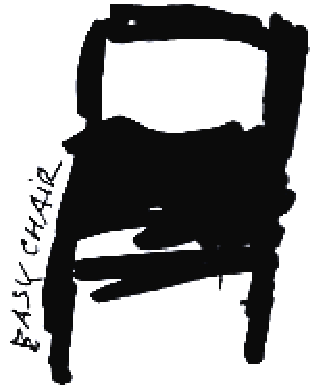
\includegraphics[width=0.2\textwidth]{images/chairEC}
	\caption{Easy Chair}
	\label{fig:easychair}
	\end{centering}
\end{figure}

%------------------------------------------------------------------------------
\subsection{Front Matter}
\label{sect:front-matter}

The front matter of an {\easychair} article follows the \texttt{article}
style, augmented with the \verb+\titlerunning+ and \verb+\authorrunning+
commands for use by authors, and the \verb+\volumeinfo+ for use by editors.
For the \verb+\author+ command with multiple authors, use \verb+\and+ to
separate authors from different institutions, as done in this document.
If the authors are from the same institution they can be separated
by commas or \verb+\\+ preceding their institution.
If the order of authors from the same institution is not consecutive, follow
the same principle as for authors from the separate institutions.
Authors must set the \verb+\titlerunning+ and \verb+\authorrunning+.
%\xf{fig:author-example} is the authors' front matter of this 
%document.
Listing~\xl{lst:author-example} is the authors' front matter of this 
document.

%\begin{figure}
%\small
%\begin{verbatim}
%\title{The {\easychair} Class File \\
%Documentation and Guide, for Authors and Editors}
%\titlerunning{The {\easychair} Class File}
%
%\author{
%    Serguei A. Mokhov\thanks{Did all the difficult work}\\
%    \affiliation{Concordia University}\\
%    \affiliation{Montreal, Quebec, Canada}\\
%    \affiliation{\url{mokhov@cse.concordia.ca}}\\
%\and
%    Geoff Sutcliffe\thanks{Did numerous tests and provided a lot of suggestions}\\
%    \affiliation{University of Miami}\\
%    \affiliation{Miami, Florida, U.S.A.}\\
%    \affiliation{\url{geoff@cs.miami.edu}}\\
%\and
%    Andrei Voronkov\thanks{Masterminded EasyChair}\\
%    \affiliation{University of Manchester}\\
%    \affiliation{Manchester, U.K.}\\
%    \affiliation{\url{andrei@voronkov.com}}\\
%}
%\authorrunning{Mokhov, Sutcliffe, and Voronkov}
%
%\maketitle
%\end{verbatim}
%\normalsize
%\caption{Example front matter}
%\label{fig:author-example}
%\end{figure}

\lstdefinestyle{codeStyle}
{
	language=tex,
	frame=single,
%	basicstyle=\footnotesize,
	basicstyle=\scriptsize,
	xleftmargin=3pt,
	xrightmargin=3pt,
	captionpos=b,
	showstringspaces=false,
	showspaces=false,
	extendedchars=true,
	linewidth=1\linewidth,
	breaklines=true,
	float=phtb
}

\begin{lstlisting}[
    label={lst:author-example},
    caption={Example Front Matter},
    style=codeStyle
    ]
\title{The {\easychair} Class File \\
Documentation and Guide, for Authors and Editors}
\titlerunning{The {\easychair} Class File}

\author{
    Serguei A. Mokhov\thanks{Did all the difficult work}\\
    \affiliation{Concordia University}\\
    \affiliation{Montreal, Quebec, Canada}\\
    \affiliation{\url{mokhov@cse.concordia.ca}}\\
\and
    Geoff Sutcliffe\thanks{Did numerous tests and provided a lot of suggestions}\\
    \affiliation{University of Miami}\\
    \affiliation{Miami, Florida, U.S.A.}\\
    \affiliation{\url{geoff@cs.miami.edu}}\\
\and
    Andrei Voronkov\thanks{Masterminded EasyChair}\\
    \affiliation{University of Manchester}\\
    \affiliation{Manchester, U.K.}\\
    \affiliation{\url{andrei@voronkov.com}}\\
}
\authorrunning{Mokhov, Sutcliffe, and Voronkov}

\maketitle
\end{lstlisting}


%------------------------------------------------------------------------------
\subsection{For Editors}
\label{sect:for-editors}

If you are not a proceedings volume editor, you may safely skip this section.
The editors have a command to the starting page number, volume and issue 
numbers, etc. For example,

\begin{verbatim}
\volumeinfo
    {J. Bloe}   % editor(s)
    {1}         % No. of editors
    {CONF 2009} % event title
    {1}         % volume number
    {4}         % issue
    {134}       % starting page number
\end{verbatim}

\noindent
The command goes into the front matter of the document. The first parameter 
is the editor(s)'s name(s). 
The second parameter is the number of the editors: if there is more than one 
then the label ``(ed.)'' becomes plural ``(eds.)''.
If you do not require volume information for your proceedings, simple do not use the command.
If you don't have either the volume number or issue fields, enter $0$
(zero) in the corresponding parameters.
The rest of the parameters are self-explanatory.

%------------------------------------------------------------------------------
\subsection{Page Numbering}
\label{sect:page-numbering}

Page numbers are at the bottom of every page. 
Authors must leave the page numbers in as-is. 
When the proceedings are prepared, the volume editors will insert the page 
numbers (see \xs{sect:for-editors}).

%------------------------------------------------------------------------------
\subsection{Section Headings}
\label{sect:section-headings}

Section and paragraph headings in {\easychair} are invoked via the standard 
commands, such as
\verb+\section+,
\verb+\subsection+,
\verb+\subsubsection+, and
\verb+\paragraph+.
Generally, every non-trivial word must be capitalized according to 
general capitalization guidelines. 
% \cite{please-add-a-reference-to-any-good-general-resource-for-capitalization}.
Paragraph headings must have a trailing period.
See the examples in this document, e.g., \xs{sect:typesetting} is a
section, this (\xs{sect:section-headings}) is a subsection, and 
\xs{sect:subsubsection-headings} is a subsubsection.

%------------------------------------------------------------------------------
\subsubsection{Subsubsection Header}
\label{sect:subsubsection-headings}

This is a subsubsection. 

\paragraph{Paragraph header.}

This is a paragraph. 
One way of saving space when hyper-references are not essential is to 
use paragraphs instead of subsubsections.

%------------------------------------------------------------------------------
\subsection{Mathematics}
\label{sect:mathematics}

Mathematics can be done inline for simple things, e.g., an equation
$x = 0$, possibly with super and subscripts, e.g., $x^2_k \approx 27$,
Greek letters, e.g., $\alpha \cup \Theta \ne \gamma$, etc.
Larger formulae must be done using {\tt \verb|\|[}~~{\tt \verb|\|]}
bracketing, e.g.,
\[
\int_{0}^{1} x dx = \left[ \frac{1}{2}x^2 \right]_{0}^{1} = \frac{1}{2}
\]
or using {\tt \verb|\|begin\{equation\}} and {\tt \verb|\|end\{equation\}} for
numbered equations, e.g.,
\begin{equation}
e^x = \sum_{n=0}^\infty \frac{x^n}{n!} = \lim_{n\rightarrow\infty} (1+x/n)^n
\end{equation}

Use {\tt \verb|\|begin\{align*\}} and {\tt \verb|\|end\{align*\}} (or without
the {\tt *} include number) to align equations, e.g.,
\begin{align*}
x^2 + y^2 &= 1 \\
y &= \sqrt{1 - x^2}
\end{align*}

Fonts, using \verb|\matcal| and others can also be used in the math mode: $\mathcal{ALC}$.

%------------------------------------------------------------------------------
\subsection{Tables}
\label{sect:tables}

\xt{tab:ltbexample} shows an example of a table of data that was
conveniently available (i.e., the data has nothing to do with {\easychair}).

\begin{table}[htp]
	\begin{centering}
		\begin{tabular}{lrrrrrrrr}
		\hline
		ATP System            & LTB & Avg  &Prfs & SOTA & \multicolumn{1}{c}{$\mu$} & CYC & MZR & SMO \\
		                      & /100& time & out & Con. & Eff. & /35 & /40 & /25 \\
		\hline
		Vampire-LTB 11.0      &  69 & 24.5 &  69 & 0.37 & 28.1 &  23 &  22 &  24 \\
		iProver-SInE 0.7      &  67 & 76.5 &   0 & 0.36 &  8.8 &  28 &  14 &  25 \\
		SInE 0.4              &  64 & 75.3 &  64 & 0.32 &  8.5 &  26 &  13 &  25 \\
		leanCoP-SInE 2.1      &  35 &110.8 &  35 & 0.23 &  3.2 &  23 &   1 &  11 \\
		E-LTB 1.1pre          &  18 & 63.4 &   0 & 0.21 &  2.8 &   7 &   9 &   2 \\
		EP-LTB 1.1pre         &  18 & 77.8 &  18 & 0.21 &  2.3 &   7 &   9 &   2 \\
		E-KRH'-LTB 1.1.3      &   0 &   -- &  -- &   -- &   -- &   0 &   0 &   0 \\
		\hline
		\end{tabular}
		\caption{LTB division results}
		\label{tab:ltbexample}
	\end{centering}
\end{table}

%------------------------------------------------------------------------------
\subsection{References}
\label{sect:references}

References must be provided in a {\tt .bib} file, so that \BibTeX\ can
be used to generate the references in a consistent style in a volume.
The preferred styles are {\tt plain} and {\tt alpha}.
For example, the references for this paper are generated from the
lines
\begin{verbatim}
    \bibliographystyle{plain}
    \bibliography{easychair}
\end{verbatim}
and a way to compose the entires, e.g. citing this class style~\cite{easychair-latex-class}
is below:
\tiny
\begin{verbatim}
    @misc
    {
      easychair-latex-class,
      author       = {Serguei A. Mokhov and Geoff Sutcliffe and Andrei Voronkov},
      title        = {The {\sf easychair} Class File Documentation and Guide,
                      for Authors and Editors},
      year         = {2008--2010},
      howpublished = {[online]},
      note         = {Available at \url{http://easychair.org/easychair.zip}}
    }
\end{verbatim}
\normalsize

%------------------------------------------------------------------------------
\section{Installation and Usage Instructions}
\label{sect:installation-usage}

%------------------------------------------------------------------------------
\subsection{Installation}

The ``installation'' of the {\easychair} document class is easy.
Download the \texttt{easychair.zip} package 
from \url{http://www.easychair.org/easychair.zip}
and unzip it in the directory where you will prepare your paper.
You will get the following files, out of which you may need to keep only 
the \texttt{easychair.cls} style class if you are familiar with the rest 
of the files and do not require them to get started.
We are also working to make {\easychair} available from CTAN \cite{ctan},
such that it can be installed with the popular \TeX Live \cite{texlive} and
{\miktex} \cite{miktex} \LaTeX package management systems.

\begin{itemize}
\item
\texttt{easychair.cls} -- the class file that this is all about.

\item
\texttt{easychair-letter.pdf} -- the PDF version of this guide rendered using 
the \texttt{letterpaper} option, 
and 
\texttt{easychair-a4.pdf} -- the PDF version of this guide rendered using 
\texttt{a4paper} option.

\item
\texttt{easychair.tex} -- the {\LaTeX} source of this guide, 
and
\texttt{easychair.bib} -- the supporting bibliography entries found starting 
on page~\pageref{sect:bib}.

\item
{\makefile} -- a ``project'' file for \texttt{make}, to automate compilation of 
this document on UNIX/Linux-like platforms,
and
\texttt{easychair.tcp} -- a ``project'' file for {\texniccenter}, to automate
compilation of this document on Windows. 
See \xs{sect:compiling}.

\item
\texttt{logoEC.pdf} -- the PDF version of the EasyChair logo rendered in
Figure~\ref{fig:easychair-logo},
\texttt{chairEC.pdf} -- the PDF version of the easy chair rendered in 
Figure~\ref{fig:easychair},
and
\texttt{throneEC.jpg} -- the JPG version of the easy throne rendered in 
Figure~\ref{fig:easythrone}.

\end{itemize}

%------------------------------------------------------------------------------
\subsection{Required Packages}

The {\easychair} class relies only on packages deemed standard and shipped by
most {\LaTeX} distributions in the worlds of Linux (current \texttt{texlive} \cite{texlive}
or older \texttt{tetex}), MacOS X,
and Windows (via Cygwin or {\miktex}).
If for some reason your distribution is old or doesn't have the packages
listed below, you can always obtain a copy from CTAN \cite{ctan}.

\begin{itemize}
\item
\texttt{inputenc} \cite{inputenc-package} -- with the default option
\texttt{utf8}, primarily to allow for UTF-8 characters.

\item
\texttt{url} \cite{url-package} (included also by \texttt{hyperref} automatically) -- to provide URL rendering support for the
monospaced font, which takes care of special characters as well as line 
wrapping.

\item
\texttt{hyperref} \cite{hyperref-package} -- to allow hyperlinking of URLs and
cross references within an article.
Its options are set to either \verb+letterpaper+ or \verb+a4paper+, depending
on the \verb+\documentclass+ options.

\item
\texttt{graphicx} \cite{graphicx-package} -- the standard package for rendering
PNG, JPG, and PDF graphic images, primarily in \texttt{figure} environments.

\item
optional \texttt{mathptmx} \cite{mathptmx-package} -- Times base font for compactness
(use with the \texttt{withtimes} {\easychair} option).

\item
\texttt{helvet} \cite{helvet-package} -- Helvetica as {\sf sans-serif}.

\item
\texttt{listings} \cite{listings-package} -- to allow highlighted source code 
listing styles.

\item
\texttt{latexsym} \cite{latexsym-package} -- to provide common math and other 
symbols.

\item
\texttt{amsthm} \cite{amsthm-package} -- to provide {\AmS} theorem-like 
environments.

\item
\texttt{empheq} \cite{empheq-package} -- to provide equation environments, etc.

\item
\texttt{geometry} \cite{geometry-package} -- to set {\easychair} margins, 
outlined in Section~\ref{sect:generalities}.

\item
\texttt{lastpage} \cite{lastpage-package} -- to allow computationally
referencing the last page.

\item
\texttt{fancyhdr} \cite{fancyhdr-package} -- for running heads.

\item
\texttt{footmisc} \cite{footmisc-package} -- to ensure that footnotes are
always at the bottom.

\item
optional \texttt{makeidx} \cite{makeidx-package} -- for index generation
(use with the \texttt{thesis} {\easychair} option).

\item
\texttt{eso-pic} \cite{eso-pic-package} -- for draft versions and checking page
overlflows vs. a border drawn aroun the headers, footers, and the main body of
the article.

\end{itemize}

%------------------------------------------------------------------------------
\subsection{Recommended Packages}
\label{sect:recommended-packages}

Here is a list of some packages that this guide's authors have experimented 
with, and which are suitable for inclusion if needed by article authors.
These packages must be loaded using \verb+\usepackage+.
In general, authors may use any standard packages provided they do not change
the basic layout and font settings established by the {\easychair} class.
Such packages must be provided with the submission of articles.

\begin{itemize}
\item
\texttt{rotating} \cite{rotating-package} -- to rotate floats (figures and
tables) on the page, when wide tables or figures do not fit in portrait layout.

\item
\texttt{pdflscape} \cite{pdflscape-package} -- similar to \texttt{rotating}, 
but also allows rotating text to make it conveniently viewable in a PDF 
viewer that supports individual rotated pages.
A possible disadvantage is that a page break is forced, which may create
gaps before or after the landscape page.

\item
\texttt{algorithm2e} \cite{algorithm2e-package} -- provides a figure-like
algorithm environment for formal algorithm presentation with highlighting.

\end{itemize}

%------------------------------------------------------------------------------
\subsection{Compiling}
\label{sect:compiling}

\texttt{pdflatex} \cite{pdflatex-instructions} is the preferred tool for
producing PDF files with {\easychair} class documents.
The author kit (\texttt{easychair.zip}) includes some minimal automation 
that authors can use at their discretion.

\begin{itemize}
\item
Linux and UNIX-like platforms (also works under Cygwin and MacOS X):
A {\makefile} is provided for the GNU \texttt{make} \cite{gmake} utility,
so this document can be compiled by typing \texttt{make} at the terminal 
prompt (on the systems where both GNU and non-GNU versions of \texttt{make} 
are installed, one may need to use \texttt{gmake}).

\item
Microsoft Windows:
{\texniccenter} \cite{texniccenter} or {\latexeditor} \cite{led} and
{\miktex} \cite{miktex} as their backend are common tools
for {\LaTeX} processing under Microsoft Windows. 
The former provide a GUI front-end to {\LaTeX}, and the latter is the 
Windows native-compiled binaries and standard packages with 
a comprehensive package update tool. 
The \texttt{easychair.tcp} project file is provided for {\texniccenter} users,
as well as \texttt{easychair.lpr} for {\latexeditor} users.

\item
MacOS X:
TeXShop \cite{texshop} is a tool for {\LaTeX} processing under Mac OS X.
It provides a GUI front-end to {\LaTeX}. The backend can be installed
through the \texttt{fink} \cite{fink} repository or the Darwin Ports.

\end{itemize}

%------------------------------------------------------------------------------
\subsection{Bug Reports}
\label{sec:bug-reports}

Please report bugs, errors, and omissions you find with the {\easychair} 
class to its primary author and current maintainer, Serguei Mokhov,
at \url{mokhov@cse.concordia.ca}. 
Any {\em constructive} feedback is always welcome.

%------------------------------------------------------------------------------
\section{Conclusion}
\label{sect:conclusion}

An article that occupies approximately 15 LNCS-formatted pages, using the 10pt 
base font size, takes up approximately 14 {\easychair} pages, using the 11pt
base font size (both using Computer Modern as a base font).

%------------------------------------------------------------------------------
\subsection{Future Work}
\label{sect:future-work}

We plan to further strengthen the {\easychair} class and promote it for 
electronic publishing for EasyChair-powered conferences and workshops,
and take over the world, as shown in Figure~\ref{fig:easythrone}.

\begin{figure}[htb!]
	\begin{centering}
	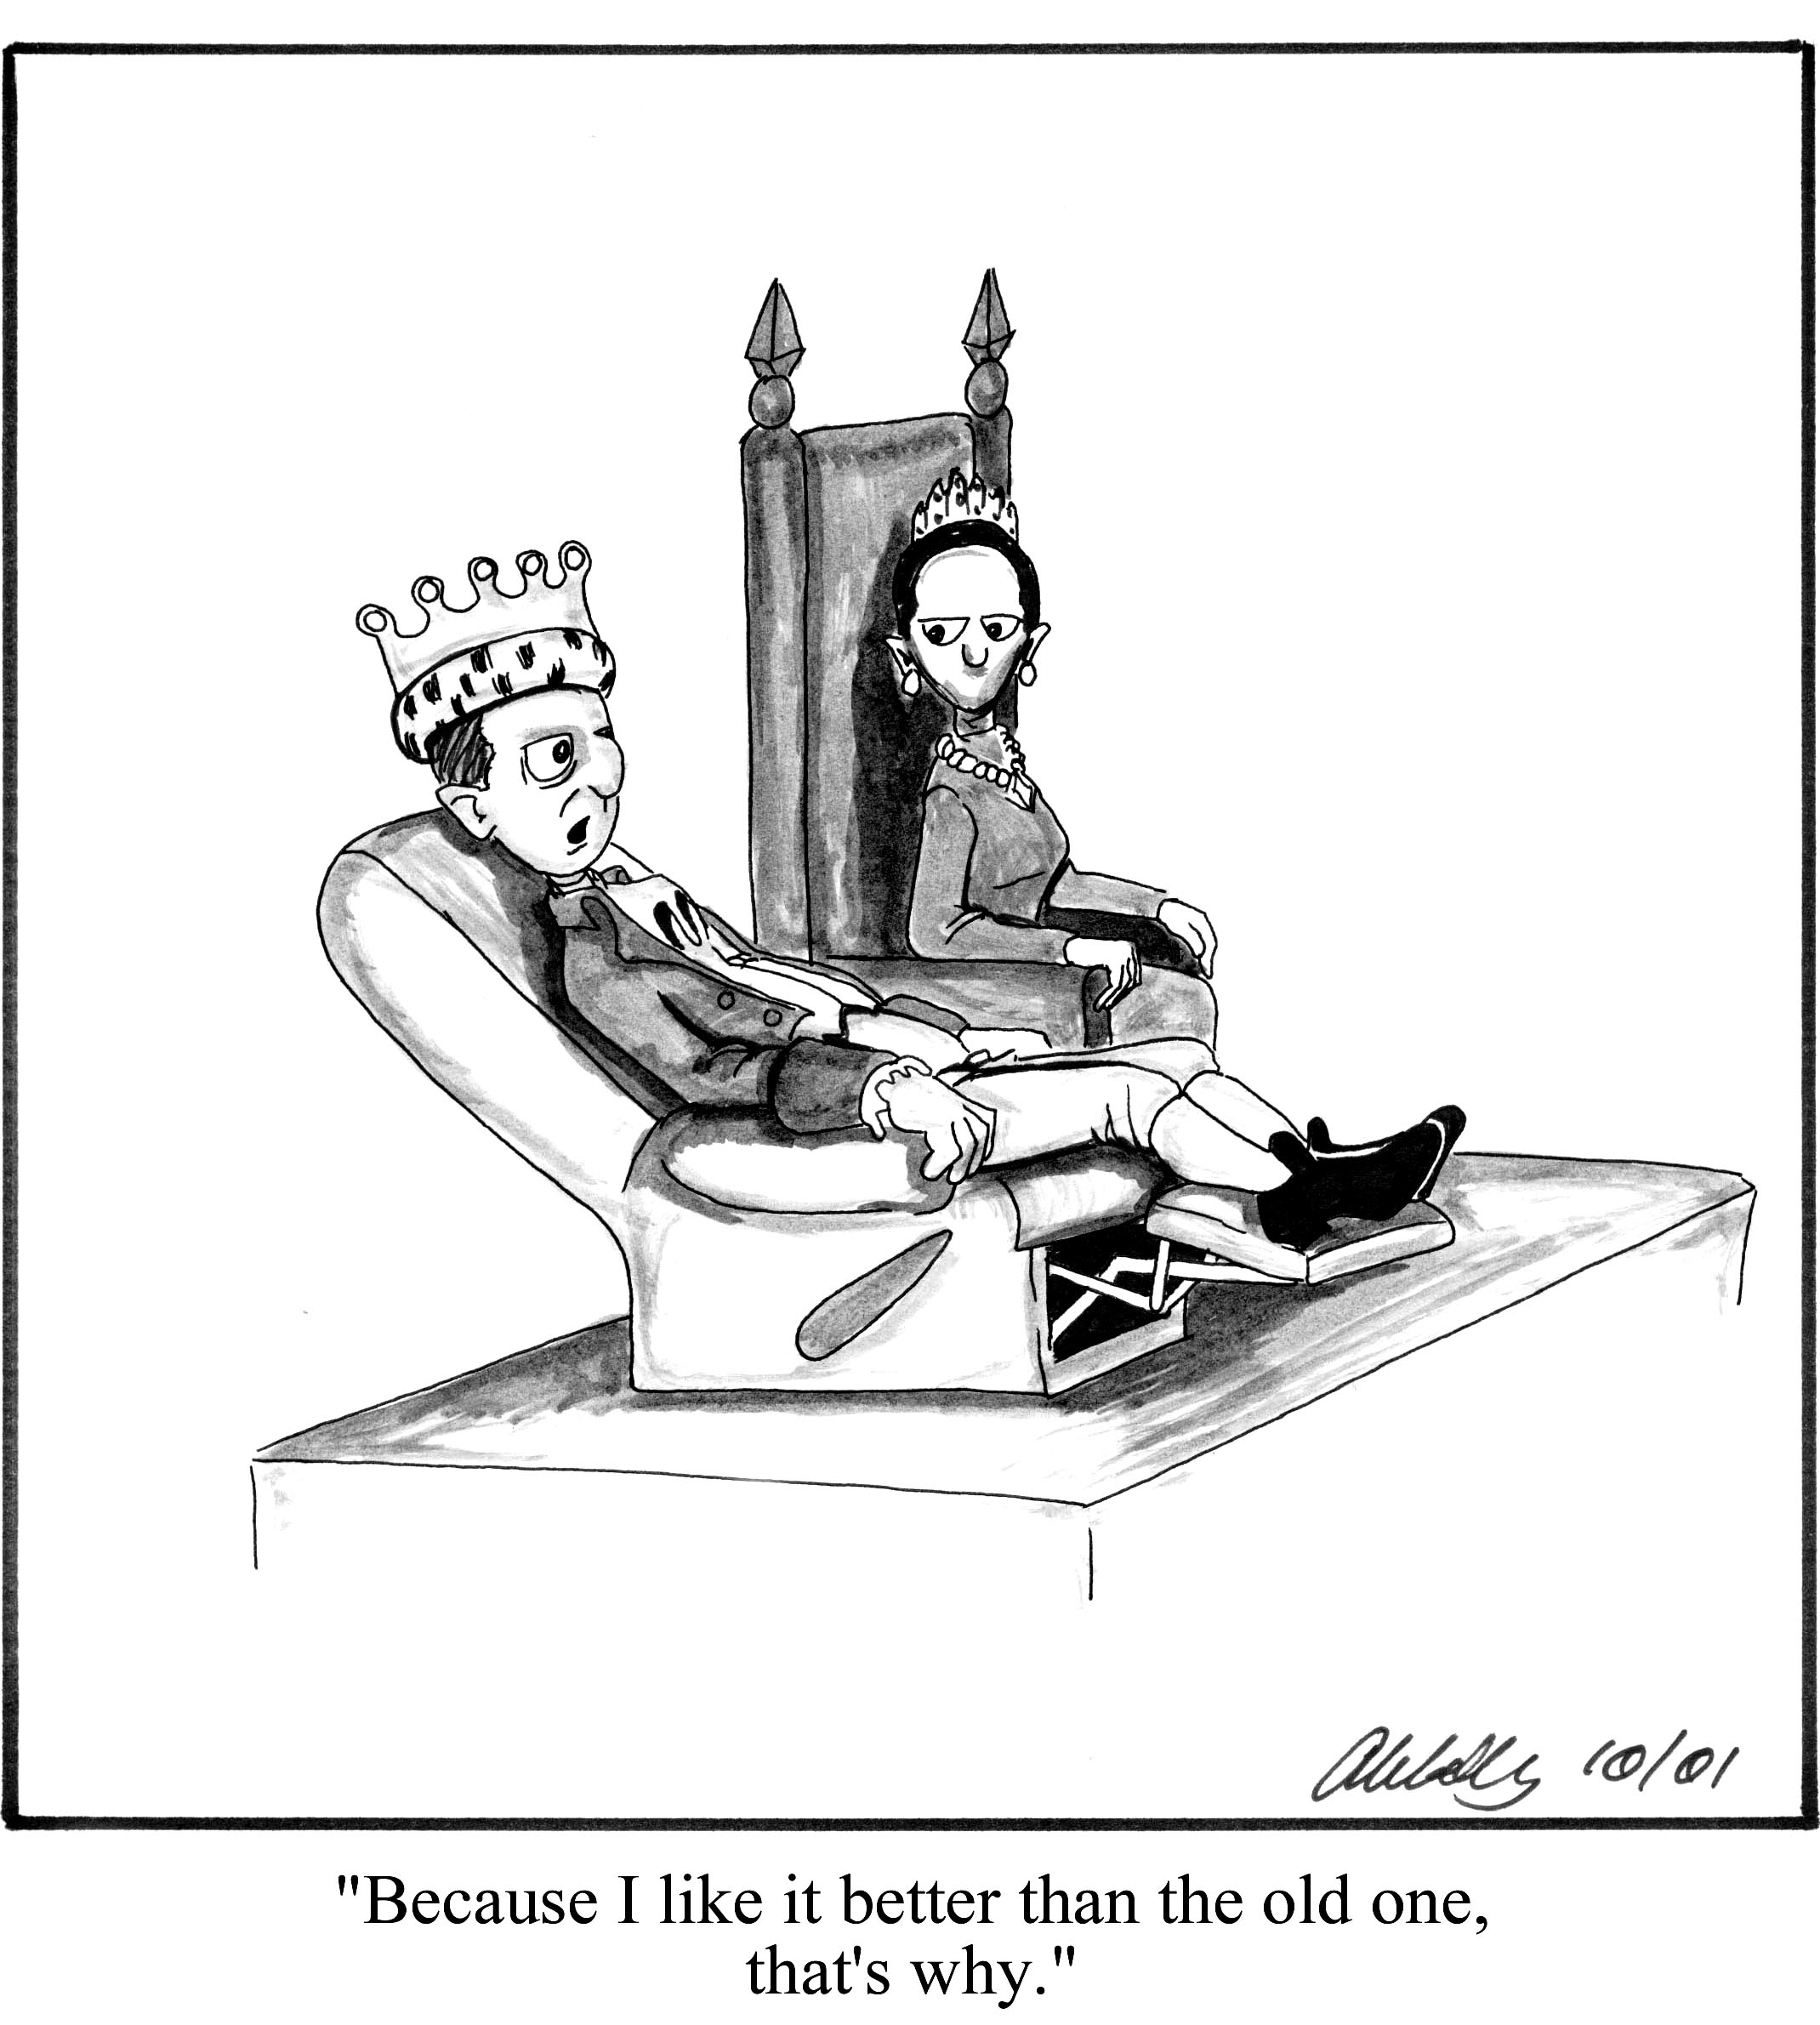
\includegraphics[width=0.5\textwidth]{images/throneEC.jpg}
	\caption{Easy Throne}
	\label{fig:easythrone}
	\end{centering}
\end{figure}

%------------------------------------------------------------------------------
\subsection{Acknowledgments}
\label{sect:acks}

\begin{itemize}
\item
Aleksander Kosenkov for the graphics that are used here, and the EasyChair 
website~\cite{easychair}.

\item
The CTAN \cite{ctan} and {\LaTeX} communities \cite{texniccenter,miktex}.

\item
Leslie Lamport for {\LaTeX} \cite{lamport-latex}.

\item
Peter Grogono for his neat kickstart {\LaTeX} introduction \cite{grogono2001}.

\item
Guilin Qi, Jasmin Christian Blanchette, Leslie Lamport, Uwe Pfeiffer, and others for constructive feedback on the style,
most of which got incorporated into the version 2 of the class style.

\end{itemize}

%------------------------------------------------------------------------------
\subsection{History}
\label{sect:history}

\begin{itemize}
\item
{\easychair} version 3.0 -- May 2011, changed to use a 10pt font.

\item
{\easychair} version 2.0 -- April 2010

\item
{\easychair} version 1.0 -- June 2008, initial release, used in ESARM'08 \cite{esarm-08,esarm-08-proceedings}
and 5 other workshops \cite{easychair}.

\end{itemize}

%------------------------------------------------------------------------------
% Refs:
%
\nocite{demo-hour-acm-interactions-jul-aug-2014}
\label{sect:bib}
\bibliographystyle{plain}
%\bibliographystyle{alpha}
%\bibliographystyle{unsrt}
%\bibliographystyle{abbrv}
\bibliography{project-report}

%------------------------------------------------------------------------------
\appendix
\section{{\easychair} Requirements Specification}
\label{sect:easychair-requirements}

The following high-level requirements were set for the development of 
the {\easychair} class, and were refined as development went along.

\begin{enumerate}
\item
The style should be easy to use. 
The average {\LaTeX} user should not need to read a long manual.

\item
It should be economical in space but the text should be nice-to-read.

\item
It should use fonts producing a reasonable-quality PDF.

\item
The bibliography should produce hyperlinks.

\item
Sections should produce menu sections in PDF.

\item
The text should look good on both A4 and letter paper.

\item
The style should be single-column.

\item
The print area should be convenient for printing using print-on-demand publishers.

\item
Running heads.

\item
A way to specify the first page number.

\item
A way to specify the volume name and number, and have it printed.
\end{enumerate}


%------------------------------------------------------------------------------
% Index
\printindex

%------------------------------------------------------------------------------
\end{document}

% EOF
